\documentclass[11pt,onecolumn]{IEEEtran}

\renewcommand{\thefootnote}{$\star$}

\usepackage[arrowdel]{physics}
\usepackage{siunitx}
\usepackage{tabularx}
\usepackage{graphicx}
\usepackage{calc}
\usepackage{listings}
\usepackage[margin=0.75in]{geometry}
\usepackage{hyperref}
\usepackage{cleveref}
\usepackage{url}
\usepackage{tikz}

\author{Henry Mitchell}
\title{LoRa Setup Writeup}
\date{}

\lstset{backgroundcolor = \color{lightgray},
  basicstyle = \ttfamily \small,
  breaklines = true,
  breakatwhitespace = true,
  commentstyle = \ttfamily \color{white},
  frame = none,
  numbers = left,
  showstringspaces = false,
  upquote = false}

\begin{document}
\maketitle
\section{Initial Testing}
\subsection{Introduction}
\label{sec:intro}
The goal of this experiment was to establish communication between wireless transceivers and a wireless gateway.
This experiment implemented an approach using SX1276RF1KAS Transceivers and Arduino Uno boards, as well as a Multi-Tech Systems MultiConnect\textregistered\ Conduit\texttrademark\ gateway.
It connects the gateway and Arduino units to a network registered with \href{https://www.thethingsnetwork.org/}{The Things Network}.
%%% Local Variables:
%%% mode: latex
%%% TeX-master: "../writeup"
%%% End:


\subsection{Materials}
\label{sec:materials}
The following were used in developing this system:
\begin{itemize}
\item SX1276RF1KAS $\times$ 1
  \begin{itemize}
  \item This is the LoRa unit which transmits the data from the Arduino to the gateway
  \end{itemize}
\item 915MHz Antenna (yellow) $\times$ 1
  \begin{itemize}
  \item This is the antenna which came with the LoRa units, and is plugged into the ``HF'' port on the LoRa unit
  \end{itemize}
\item Arduino Uno board $\times$ 1
  \begin{itemize}
  \item This is the micro-controller which determines which data to collect and send
  \end{itemize}
\item USB 2.0 Type B cable $\times$ 1
  \begin{itemize}
  \item This is to connect the Arduino unit to a computer, in order to upload instructions to them
  \end{itemize}
\item Jumper Wires
  \begin{itemize}
  \item These are to connect the Arduino and LoRa unit
  \end{itemize}
\item Multi-Tech Systems MultiConnect\textregistered\ Conduit\texttrademark\ (MTCDT-LAT1-247A)
  \begin{itemize}
  \item This is the gateway to connect the LoRa network to the cloud
  \end{itemize}
\item Required Arduino libraries
  \begin{itemize}
  \item These are the \href{https://www.arduino.cc/en/Reference/SPI}{SPI library} and \href{https://github.com/matthijskooijman/arduino-lmic}{LMIC}.
  \end{itemize}

\end{itemize}

We are using the same pin mapping as in the previous section, shown in \cref{tab:pinmap}.

%%% Local Variables:
%%% mode: latex
%%% TeX-master: "../writeup"
%%% End:


\subsection{Connecting Sensors}
\label{sec:setup}
Before establishing communication between the two units, sensors must be connected.
As things currently stand, the client code is set up for two sensors.  One of these is to be connected to pin A0, and the other is to be connected to A1.
In future versions of the software, the number of sensors will not be hard-coded, but will simply allow for a plug-and-play style of use.
Additionally, any functions that will be used to process the raw data from the sensors must be edited (they are currently called \lstinline[language=C++]{fix_temp} and \lstinline[language=C++]{fix_sound}, and are in \url{arduino/client/client.ino}\footnote{All file paths are relative to the main git repository.}).
Sensors will also need to be connected to the Arduino's \SI{3.3}{\volt} and ground pins.

%%% Local Variables:
%%% mode: latex
%%% TeX-master: "../writeup"
%%% End:


\subsection{Procedure}
\label{sec:procedure}
In order to establish communication between the Arduino and the gateway, we need to prepare both components.
To prepare the gateway to act as an interface between the Arduino and the cloud, I registered it with The Things Network and followed the \href{https://www.thethingsnetwork.org/docs/gateways/multitech/aep.html}{instructions} provided by The Things Network.

Once all of the components are registered with The Things Network, we can set up our Arduino.
After logging into The Things Network's website, we need to navigate to the ``Applications'' pane.
This will allow us to get the necessary information to allow our Arduinos to join the LoRa network.
We need a device EUI, an application EUI, and an application key in order for the Arduino to join the network.
These are available on the console, as shown in \cref{fig:console}\footnote{The app key has been blurred out, as it should be kept secure to prevent new devices from being added to the network without administrator permission.}.
\begin{figure}[ht]
  \centering
  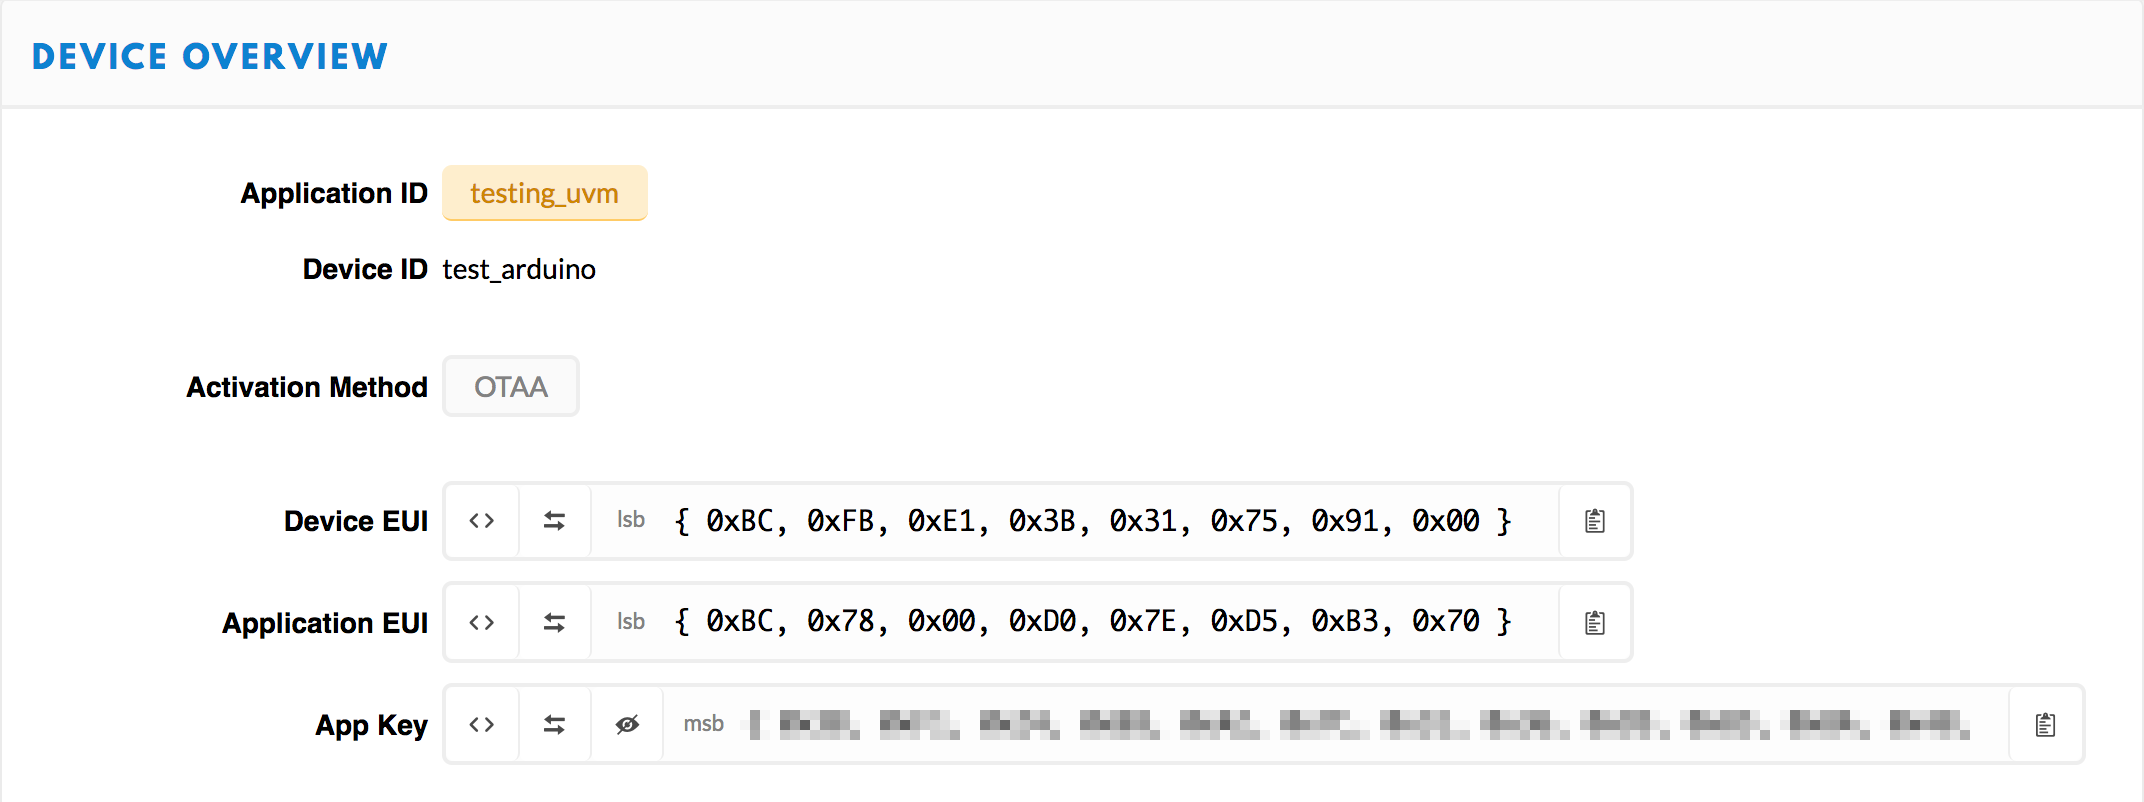
\includegraphics[width=\textwidth]{figure/console}
  \caption{The device overview from The Things Network console.}
  \label{fig:console}
\end{figure}

These get put into the over-the-air-activation (OTAA) script at \url{arduino/ttn_otaa/ttn_otaa.ino} as shown in \cref{fig:script}.
\begin{figure}[ht]
  \centering
  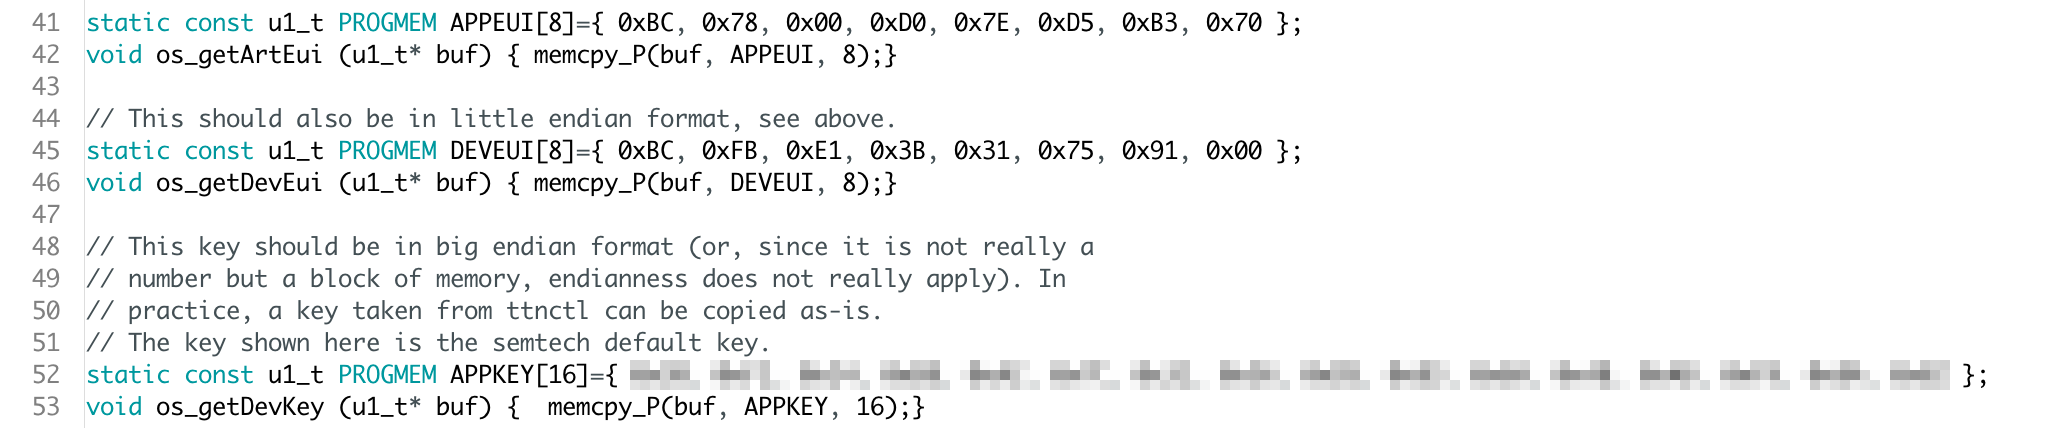
\includegraphics[width=\textwidth]{figure/script}
  \caption{The placement of the information from the The Things Network console.}
  \label{fig:script}
\end{figure}
Once these edits have been made, the script is uploaded to the Arduino, which tries to join the network established by the gateway.

%%% Local Variables:
%%% mode: latex
%%% TeX-master: "../writeup"
%%% End:


\section{Gateway Communication}
\label{sec:gateway}
\subsection{Introduction}
\label{sec:gateway:intro}
The goal of this experiment was to establish communication between wireless transceivers and a wireless gateway.
This experiment implemented an approach using SX1276RF1KAS Transceivers and Arduino Uno boards, as well as a Multi-Tech Systems MultiConnect\textregistered\ Conduit\texttrademark\ gateway.
It connects the gateway and Arduino units to a network registered with \href{https://www.thethingsnetwork.org/}{The Things Network}.
%%% Local Variables:
%%% mode: latex
%%% TeX-master: "../writeup"
%%% End:


\subsection{Materials}
\label{sec:gateway:materials}
The following were used in developing this system:
\begin{itemize}
\item SX1276RF1KAS $\times$ 1
  \begin{itemize}
  \item This is the LoRa unit which transmits the data from the Arduino to the gateway
  \end{itemize}
\item 915MHz Antenna (yellow) $\times$ 1
  \begin{itemize}
  \item This is the antenna which came with the LoRa units, and is plugged into the ``HF'' port on the LoRa unit
  \end{itemize}
\item Arduino Uno board $\times$ 1
  \begin{itemize}
  \item This is the micro-controller which determines which data to collect and send
  \end{itemize}
\item USB 2.0 Type B cable $\times$ 1
  \begin{itemize}
  \item This is to connect the Arduino unit to a computer, in order to upload instructions to them
  \end{itemize}
\item Jumper Wires
  \begin{itemize}
  \item These are to connect the Arduino and LoRa unit
  \end{itemize}
\item Multi-Tech Systems MultiConnect\textregistered\ Conduit\texttrademark\ (MTCDT-LAT1-247A)
  \begin{itemize}
  \item This is the gateway to connect the LoRa network to the cloud
  \end{itemize}
\item Required Arduino libraries
  \begin{itemize}
  \item These are the \href{https://www.arduino.cc/en/Reference/SPI}{SPI library} and \href{https://github.com/matthijskooijman/arduino-lmic}{LMIC}.
  \end{itemize}

\end{itemize}

We are using the same pin mapping as in the previous section, shown in \cref{tab:pinmap}.

%%% Local Variables:
%%% mode: latex
%%% TeX-master: "../writeup"
%%% End:


\subsection{Caveats}
\label{sec:gateway:caveats}
As things currently stand, the gateway can not be connected to a secured network.
While the network can have a WPA2 password, it can not have a firewall or any additional security measures.
You can test your internet connection from the gateway by \lstinline[language=sh]{ping}ing Google's \lstinline[language=sh]{8.8.8.8} server.
If you see results like those shown in \cref{fig:ping}, then your network is sufficiently exposed.
\begin{figure}[ht]
  \centering
  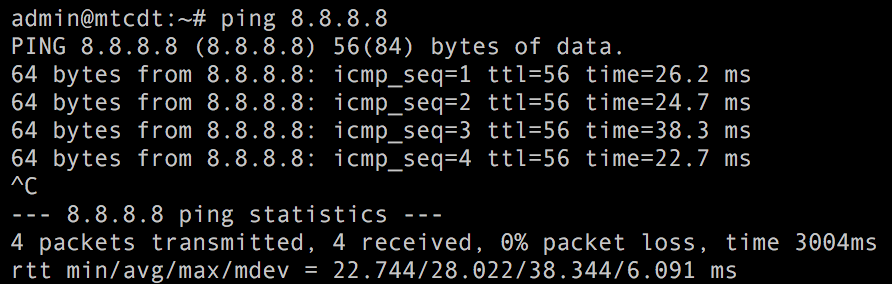
\includegraphics[width=0.5\textwidth]{figure/ping}
  \caption{The expected output of a \lstinline[language=sh]{ping 8.8.8.8} from the gateway.}
  \label{fig:ping}
\end{figure}

Additionally, as of the time of this writing, the \lstinline{config.h} file for the LMIC library is not configured for this use.
The necessary changes are as follows:
\begin{itemize}
\item Comment the line that says \lstinline[language=C]{#define CFG_eu868 1} and un-comment the line that says \lstinline[language=C]{#define CFG_us915 1}
\item Un-comment the line that says \lstinline[language=C]{#define DISABLE_INVERT_IQ_ON_RX}
\end{itemize}

%%% Local Variables:
%%% mode: latex
%%% TeX-master: "../writeup"
%%% End:


\subsection{Procedure}
\label{sec:gateway:procedure}
In order to establish communication between the Arduino and the gateway, we need to prepare both components.
To prepare the gateway to act as an interface between the Arduino and the cloud, I registered it with The Things Network and followed the \href{https://www.thethingsnetwork.org/docs/gateways/multitech/aep.html}{instructions} provided by The Things Network.

Once all of the components are registered with The Things Network, we can set up our Arduino.
After logging into The Things Network's website, we need to navigate to the ``Applications'' pane.
This will allow us to get the necessary information to allow our Arduinos to join the LoRa network.
We need a device EUI, an application EUI, and an application key in order for the Arduino to join the network.
These are available on the console, as shown in \cref{fig:console}\footnote{The app key has been blurred out, as it should be kept secure to prevent new devices from being added to the network without administrator permission.}.
\begin{figure}[ht]
  \centering
  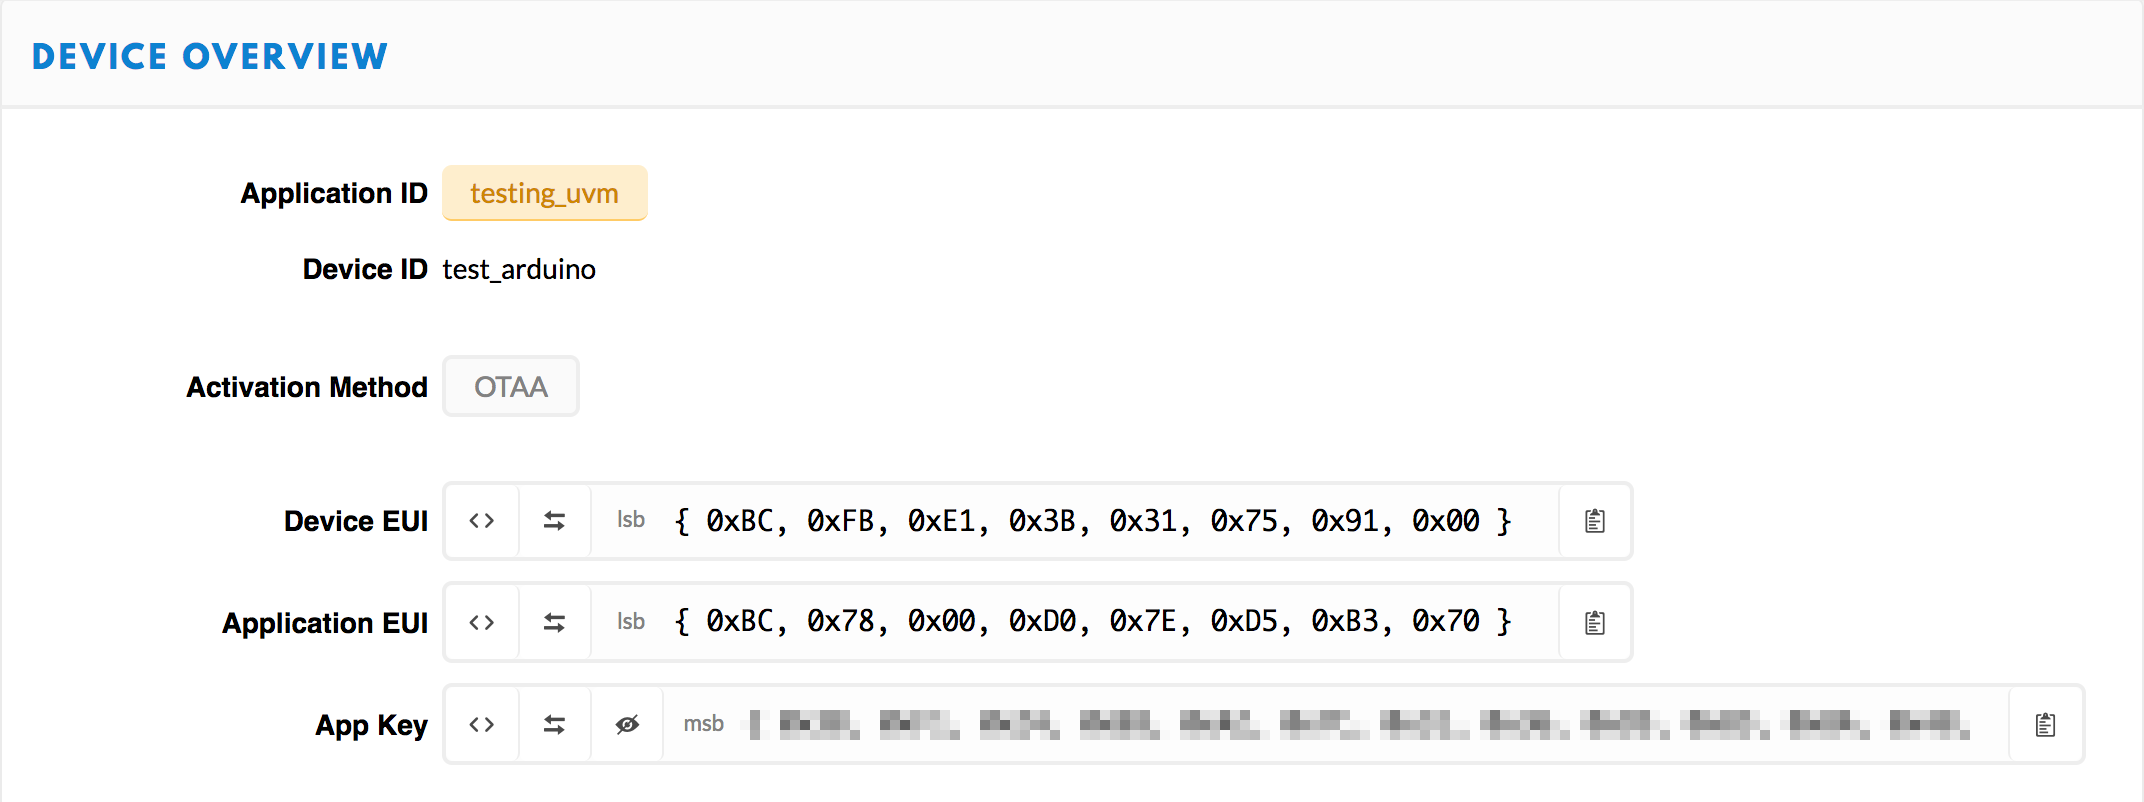
\includegraphics[width=\textwidth]{figure/console}
  \caption{The device overview from The Things Network console.}
  \label{fig:console}
\end{figure}

These get put into the over-the-air-activation (OTAA) script at \url{arduino/ttn_otaa/ttn_otaa.ino} as shown in \cref{fig:script}.
\begin{figure}[ht]
  \centering
  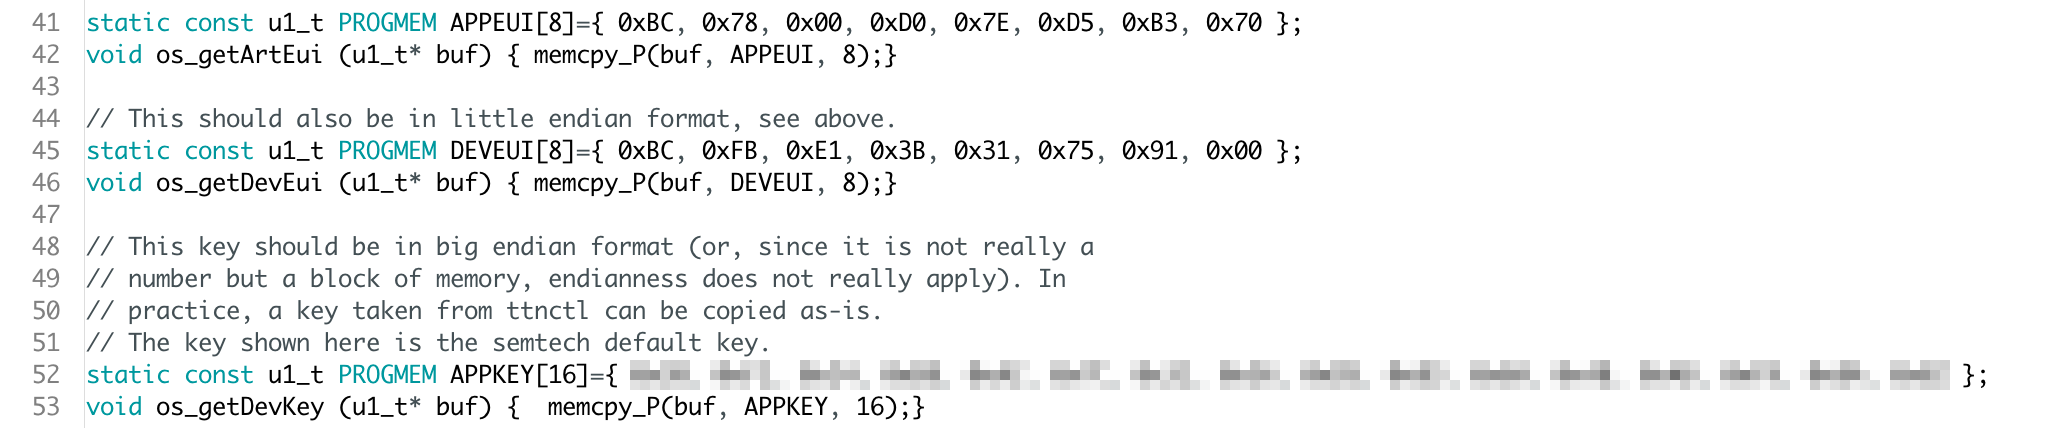
\includegraphics[width=\textwidth]{figure/script}
  \caption{The placement of the information from the The Things Network console.}
  \label{fig:script}
\end{figure}
Once these edits have been made, the script is uploaded to the Arduino, which tries to join the network established by the gateway.

%%% Local Variables:
%%% mode: latex
%%% TeX-master: "../writeup"
%%% End:


\subsection{Results}
\label{sec:gateway:results}
\subsubsection{First Iteration}
As things currently stand, the gateway is able to receive transmissions from the Arduino, but the Arduino is unable to receive the acknowledge that the gateway sends upon OTAA.
However, the gateway is receiving data from the Arduino, and forwarding said data to The Things Network, where it is accessible.
We can see the Arduino's attempts at establishing a connection in \cref{fig:gateway_serial}.
\begin{figure}[ht]
  \centering
  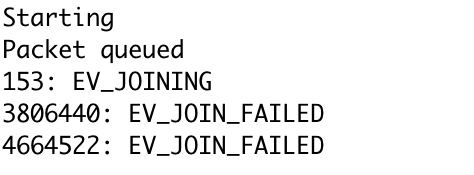
\includegraphics{figure/gateway_serial}
  \caption{The Arduino's attempts to establish a connection in the network.  Because it is not receiving the gateway's ACK signal, it is viewing its attempts as failures.}
  \label{fig:gateway_serial}
\end{figure}

However, we can see that the gateway is receiving the data that the Arduino is transmitting, because the data are appearing on The Thing Network's console.
The gateway's input and output are shown together in \cref{fig:gateway_console}, while only the data received from the Arduino are shown in \cref{fig:arduino_console}.
\begin{figure}[ht]
  \centering
  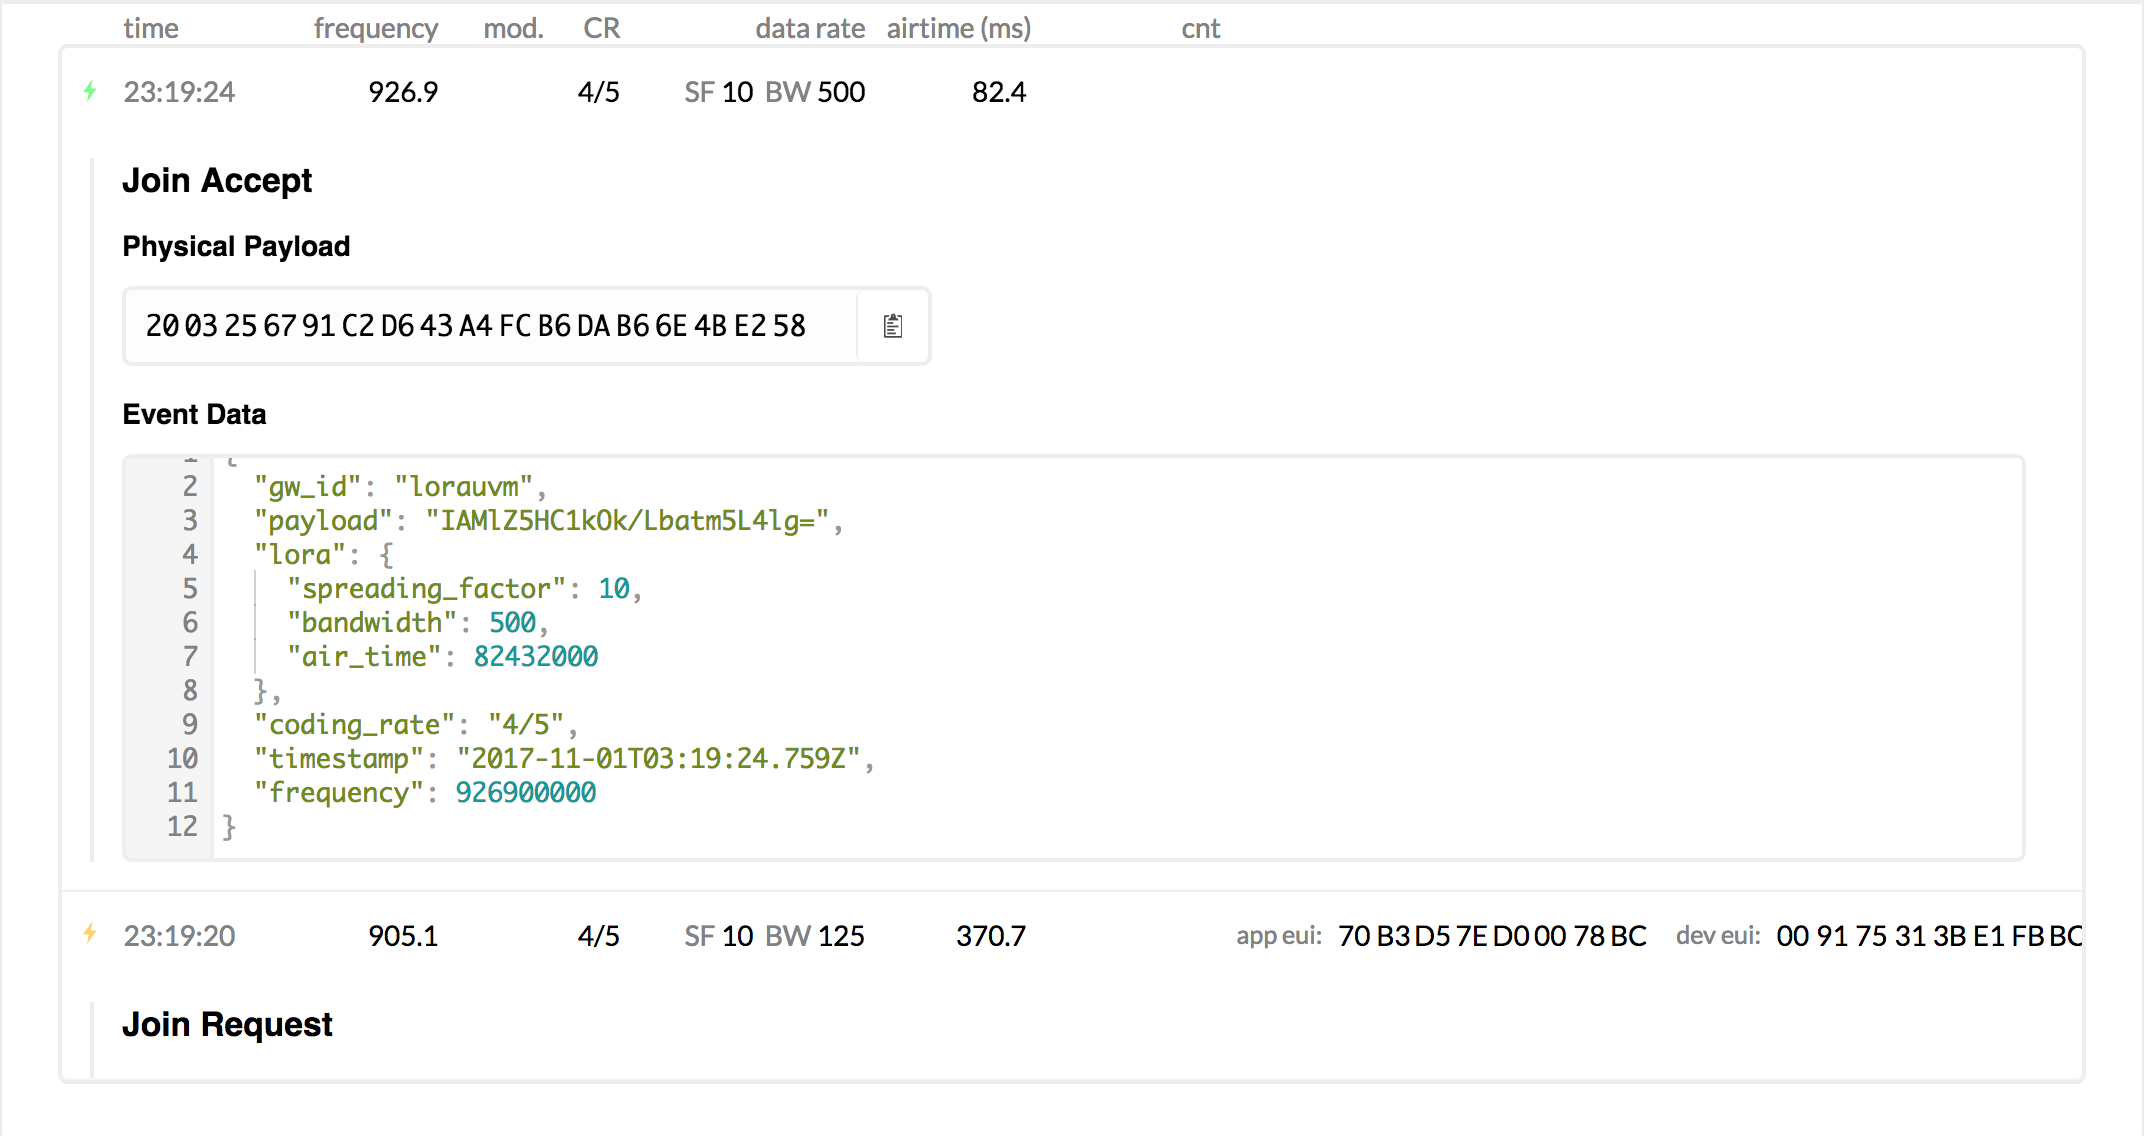
\includegraphics[width=\textwidth]{figure/gateway_console}
  \caption{The data received and transmitted by the gateway, as they appear on The Things Network's console.}
  \label{fig:gateway_console}
\end{figure}
\begin{figure}[ht]
  \centering
  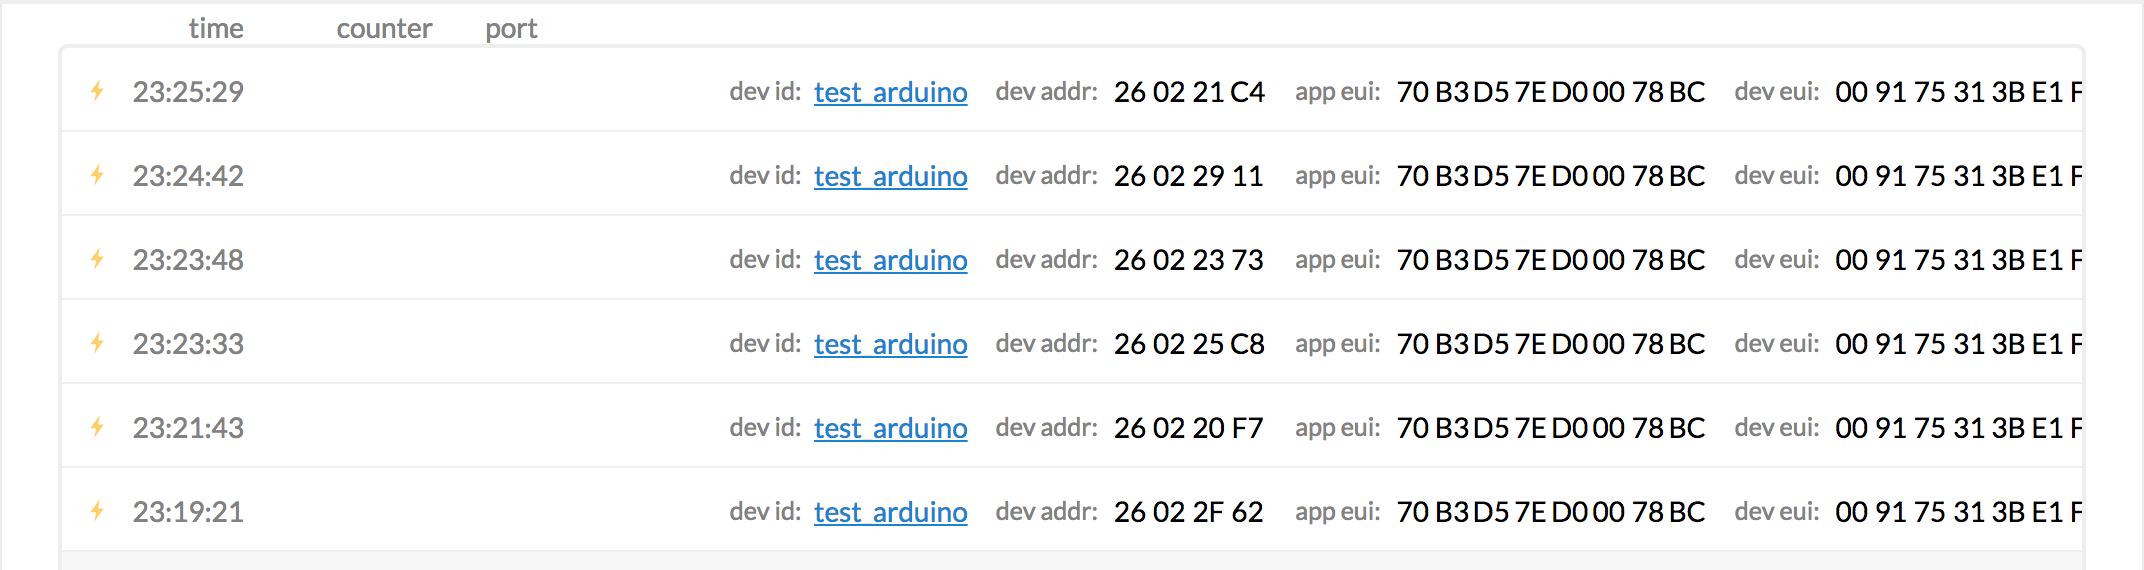
\includegraphics[width=\textwidth]{figure/arduino_console}
  \caption{The data transmitted by the Arduino, as they appear on The Things Network's console.}
  \label{fig:arduino_console}
\end{figure}

\subsubsection{Second Iteration}
After much troubleshooting, the Arduino was able to receive the acknowledge from the gateway.
This was achieved by changing the tolerance on the Arduino's clock, adding
\begin{lstlisting}[language=C++]
  LMIC_setClockError(MAX_CLOCK_ERROR * 1 / 100);
\end{lstlisting}
to the OTAA script's \lstinline[language=C++]{setup} function.
This allowed for a stable connection.

The issue with this connection is that the range is extremely limited, with a maximum of approximately \SI{20}{\meter}.

%%% Local Variables:
%%% mode: latex
%%% TeX-master: "../writeup"
%%% End:


\subsection{Discussion}
\label{sec:gateway:discussion}
The next steps are to get the Arduino to receive the ACK signal that the gateway is sending to it, and to test the range of this LoRa network.
Once we get the Arduino to receive the ACK signal, it will be able to transmit more helpful data, like that from sensors.

%%% Local Variables:
%%% mode: latex
%%% TeX-master: "../writeup"
%%% End:


\end{document}

%%% Local Variables:
%%% mode: latex
%%% TeX-master: t
%%% End: